\documentclass[10pt,a4paper]{article}
\usepackage[utf8]{inputenc} % para poder usar tildes en archivos UTF-8
\usepackage[spanish]{babel} % para que comandos como \today den el resultado en castellano
\usepackage{a4wide} % márgenes un poco más anchos que lo usual
\usepackage[conEntregas]{caratula}
\usepackage{mathtools}
\usepackage{float}
\usepackage[pdftex]{graphicx}
\usepackage{caption}
\usepackage{subcaption}
%\usepackage{Sty/algorithm2e}
\usepackage[ruled,vlined]{algorithm2e}
%Esto de abajo es para encabezado y pie de pagina
\usepackage{lastpage}
\usepackage{fancyhdr}
\usepackage{amsfonts}
\usepackage{verbatim}
\usepackage{wrapfig}
\usepackage{multirow}
\usepackage{ulem} 

\pagestyle{fancy}
%\fancyhf{} % clear all header and footer fields
%\fancyfoot[R]{\footnotesize Página \thepage\ de \lastpage\}

\cfoot{\thepage /\pageref{LastPage} }

\begin{document}

\titulo{Trabajo Práctico \#1}
\subtitulo{Sistema de inscripción Mundial de Irlanda 2017}

\fecha{\today}

\materia{Bases de Datos}
\grupo{Grupo 7}

% Pongan cuantos integrantes quieran
\integrante{Abdala Leila}{950/12}{abdalaleila@gmail.com}
\integrante{Bernaus Andres}{699/10}{andres.bernaus@hotmail.com}
\integrante{Gonzalez Alejandro}{32/13}{gonzalezalejandro1592@gmail.com}
\integrante{Romero Lucas}{440/12}{lucasrafael.romero@gmail.com}

\maketitle

\newpage
\tableofcontents

\newpage
\section{Introducci\'on}

Con motivo del Campeonato Mundial de Taekwon\-do ITF, se desea modelar e implementar la base de datos para el sistema de inscripciones del mismo. 

El objetivo principal de esta base de datos ser\'a, en primer lugar, responder a las consultas relacionadas con el proceso de inscripción en s\'i. Es decir, obtener el listado de inscriptos de las escuelas, listado de inscriptos por categoría, categorías en las que participo cada competidor, lista de equipos por país, etc. El modelo también debe permitir obtener los resultados del torneo, como por ejemplo las medallas obtenidas por cada país, puntajes de cada una de las escuelas que participaron, etc.

\section{Modelo}

A continuación veremos en detalle los distintos aspectos del problema a resolver, y como decidimos modelarlos para cumplir con los requerimientos del problema.

\subsection{Inscripciones}

Para poder participar en el Torneo, los maestros de cada escuela deberán inscribir a sus alumnos y coach's en el certamen. A partir de esto, podemos deducir al menos 3 entidades: el \textbf{maestro} los \emph{alumnos} inscriptos y los \emph{coach's}. Sin embargo, podríamos obtener una mayor cantidad de entidades dependiendo de como se interprete a alguno de ellos (alumnos inscriptos, competidores). Tomemos por ejemplo al Maestro, este podría ser modelado como una entidad con sus datos personales, el nombre de su escuela, y país como atributos; o podríamos crear la entidad \textbf{Escuela} y que esta tenga los atributos nombre y país. Permitiéndonos acceder a estos datos de manera sencilla al momento de relacionarlas con sus competidores y resultados obtenidos en la competencia.\\

Para los alumnos y coachs inscriptos decidimos modelarlos en las entidades \emph{Competidor} y \textbf{Coach} respectivamente. Utilizando como clave primaria para ambos casos el numero de certificado ITF, que asumimos, es único para cada persona. Para el caso en que los Coachs participan a la vez como Competidores, simplemente nos aseguraremos de que los datos repetidos (nombre, certificado ITF, graduación, etc) sean consistentes en ambas entidades.\\

Obteniendo de momento el siguiente DER:

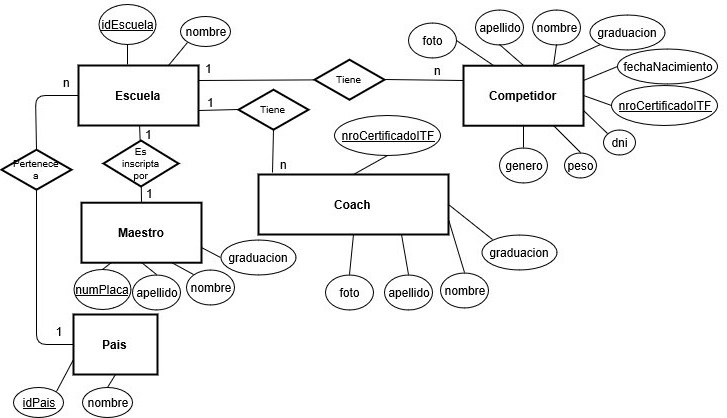
\includegraphics[scale=0.75]{inscripcion.jpg}

\newpage
\subsection{Competencias, modalidades y resultados obtenidos}

El siguiente aspecto a modelar es la participación de los alumnos y Coachs en cada competencia. Dado que cada competidor debe estar acompañado por un Coach al momento de competir, decidimos modelarlo como una relación ternaria 1-n-m entre las entidades Coach, Competidor y Competencia respectivamente. Y como se deben tener en cuenta las restricciones de cada tipo de competencia para con sus participantes; se creo también la entidad \textbf{Modalidad}, que tendrá como atributos las distintas restricciones para cada categoría, como por ejemplo edad mínima y máxima, peso, graduación, etc.\\

Para el caso de combates por grupo decidimos crear otra relacion ternaria entre las entidades \textbf{Coach}, \textbf{Equipo}, y \textbf{Competencia}. La entidad Equipo se relacionara a su vez de forma parcial con la entidad Competidores, debido a que no todos los competidores participaran en la modalidad de combate por grupos. Ademas se deberá constatar que todos los integrantes que formen un equipo  sean del mismo sexo, y pertenezcan a la misma escuela.\\

Finalmente agregamos dos interrelaciones n a m entre las Competencias y sus competidores (o equipos). Estas relaciones almacenaran los resultados de los participante de cada una de las competencias en las que hayan participadon.\\

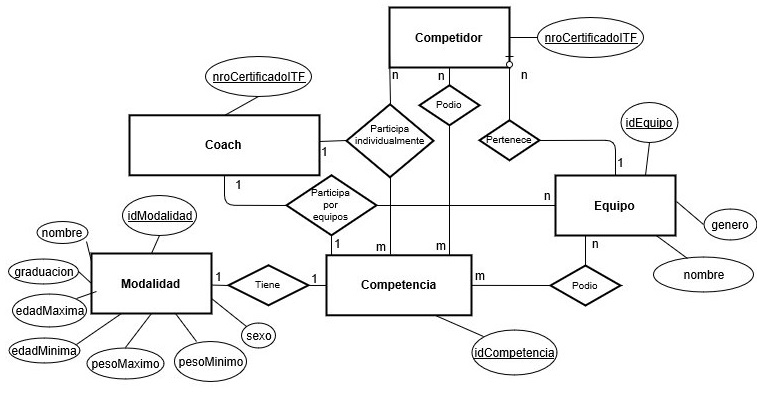
\includegraphics[scale=0.75]{competenciaDiag.jpg}


\subsection{Arbitraje}

Por ultimo, nuestro modelo debe ser capaz de obtener los árbitros de cada país que participaron en el torneo, y ademas la lista de árbitros que participaron como ``Arbitro Central'' en las modalidades de combate.\\

Para modelar esto, simplemente definimos las entidades: 
\begin{itemize}
\item \textbf{Arbitro} la cual contendrá toda la información de cada uno de los árbitros que participan, incluyendo el país al que pertenece.
\item \textbf{Rol} que tendrá las posibles funciones que pueden ejercer los árbitros del torneo. Es decir, arbitro central, presidente de mesa, juez o suplente.
\end{itemize}
Luego cada arbitro habrá realizado un rol determinado sobre un ring, formando entonces una relación 1 a n con la entidad rol; y ademas habr\'a participado en varias competencias. Lo que se reduce a una relación n a m entre las entidades \textbf{Competencia} y \textbf{Arbitro}.\\

Si se quieren consultar los ``Árbitros Centrales'' de las modalidades de combate, lo único que debemos hacer es obtener los árbitros que ejercieron dicho rol, y comprobar si existe una entrada que los relacionen con alguna de las competencias con modalidad de combate.\\

En el caso de la consulta de árbitros por país, se puede realizar filtrando todo los elementos de la entidad Árbitros que pertenezcan al país deseado. \\

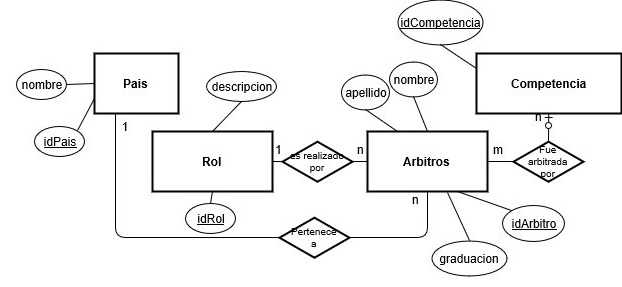
\includegraphics[scale=0.75]{arbitroDiag.jpg}

\subsection{Diagrama Entidad Relaci\'on}

A partir de todas los puntos presentados anteriormente obtenemos el siguiente DER: (Notar que únicamente mostraremos las entidades sus interrelaciones y claves primarias para observar todo el diagrama con mayor claridad)\\

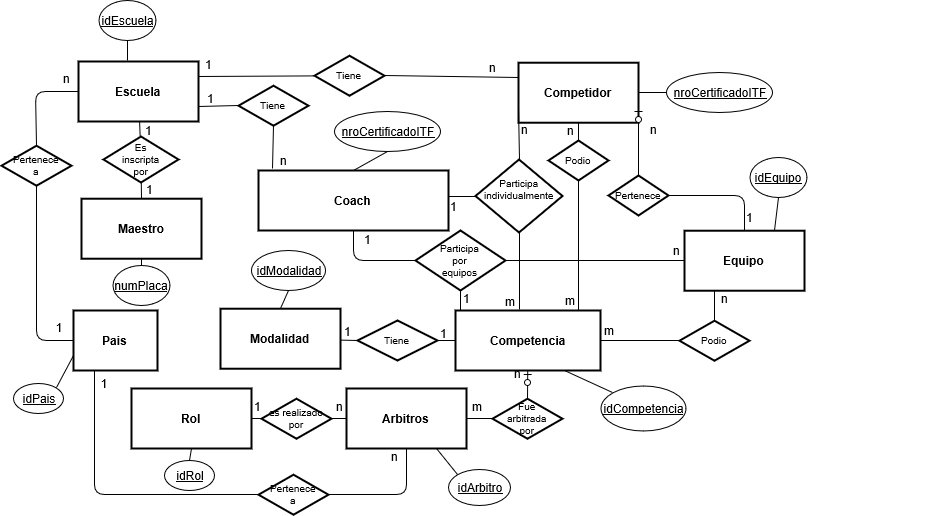
\includegraphics[scale=0.55]{der.jpg}

\section{Modelo Relacional}

\section{Conclusión}

\end{document}
